\chapter{Introdução}

Qualquer pessoa, que necessite se deslocar pela cidade, tem contato com o trânsito em vias urbanas e tem sua rotina influenciada pelo mesmo, seja dirigindo um carro, andando de ônibus ou atravessando ruas. O conceito de trânsito pode ser aplicado tanto para pedestres como para motoristas (e passageiros), pois ele representa a utilização das vias por pessoas, veículos e animais, isolados ou em grupos, conduzidos ou não, para fins de circulação, parada, estacionamento e operação de carga ou descarga \cite{lei}.
%[http://www.planalto.gov.br/ccivil_03/LEIS/L9503.htm]

Com essa definição, é evidente que as vias urbanas são um espaço compartilhado entre diversos automóveis e pedestres, de modo que é necessário estar atento a dois parâmetros: segurança e redução de riscos, e controle e gerenciamento do fluxo das vias.

A questão da segurança é importante pois o trânsito seguro é um direito de todos e um dever dos órgãos e entidades do Sistema Nacional de Trânsito \cite{manual3}, %[Manual de direção defensiva DENATRAN]
e sem devido controle e sinalização de vias, existe um aumento considerável de riscos de acidentes em locais de conflito entre movimentos de veículos, em locais de cruzamento de vias, ou entre veículos e pedestres, em locais de travessia.

O controle de fluxo é importante, pois com o aumento constante das frotas de veículos nos centros urbanos, a tendência é a sobrecarga da capacidade das vias mais movimentadas. A capacidade de uma via pode ser descrita como o fluxo máximo de veículos permitidos, sem que haja atrasos significativos nos tempos de viagens. Uma sobrecarga na capacidade de uma via resulta em congestionamentos, que trazem pontos negativos ao dia a dia das pessoas envolvidas, como exposição a potenciais perigos urbanos, aumento indesejável do tempo de viagem e aumento de estresse.

Por questões de limitações de espaço urbano, não é possível a expansão indefinida da largura das vias, para comportar mais veículos, por isso, para evitar, ou reduzir, o congestionamento, é necessária a utilização de sinalização e equipamentos eficientes e tecnológicos, com o intuito de realizar algum tipo de controle, a fim de garantir a segurança de todos e a organização dos fluxos, assim como a redução de riscos de acidentes.

\section{Motivação}

O Brasil possui 97 milhões de veículos, dos quais 5.4 milhões chegaram às ruas no ano de 2017, desse número quase 90\% é composto por veículos que circulam diariamente em vias urbanas, como automóveis, motocicletas e ônibus. Essa quantidade vem crescendo a cada ano, com uma média de 3.84 milhões de novos veículos por ano, nos últimos cinco anos. %[http://www.denatran.gov.br/index.php/estatistica/610-frota-2017]. 
Uma grande quantidade de veículos em circulação pode facilmente sobrecarregar a capacidade das vias urbanas, trazendo consequências para o trânsito.

Pesquisas realizadas no começo do ano de 2018 mostraram que, em horários de pico, o trânsito nas principais capitais brasileiras pode resultar em tempos de viagens até 77\% mais demorados que o usual\cite{recife}, %[http://jc.ne10.uol.com.br/blogs/deolhonotransito/2018/03/27/recife-capital-com-o-transito-mais-lento-do-pais-de-novo/]
isso é uma consequência da quantidade de veículos nas ruas. Além disso, existem pesquisas relacionando o trânsito como um gerador de estresse na população, principalmente nos em condutores veiculares, e o estresse como uma das principais causas das agressividades no trânsito \cite{stress}\cite{stress2}.  %[https://www.researchgate.net/profile/Vinicius_Ferreira3/publication/237480019_Comportamentos_no_transito_e_causas_da_agressividade/links/02e7e528bc018b2f72000000/Comportamentos-no-transito-e-causas-da-agressividade.pdf] [https://singep.org.br/6singep/resultado/406.pdf] [http://www2.fm.usp.br/gdc/docs/iof_89_estressetrans.pdf].

Com o intuito de reduzir riscos e aumentar a organização das vias, é utilizada a sinalização de trânsito. A sinalização de trânsito é o elemento de ligação entre o técnico, o usuário da via, motoristas e pedestres e os agentes de fiscalização. Seu objetivo principal é o de garantir a utilização adequada da via, no sentido da segurança e fluidez do tráfego como um todo. Para atingir este objetivo, é necessário que a sinalização contenha uma mensagem clara e inconfundível e que seja plenamente visível. Desse modo, iniciou-se a padronização dos elementos responsáveis por realizar a sinalização, em cores, formatos, dimensões e critérios de utilização\cite{CET}. %[http://www.cetsp.com.br/media/391986/msuvol01_introducaorev01.pdf]. 
O foco deste trabalho é a sinalização semafórica das vias urbanas.

\begin{figure}[ht]
    \begin{center}
    \subfloat[Semáforo veicular]{\label{veicular}
    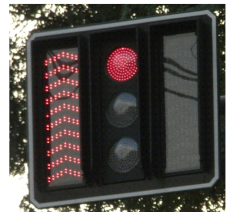
\includegraphics{figuras/semaforo.PNG}}
    \subfloat[Semáforo de pedestres]{\label{pedestre}
    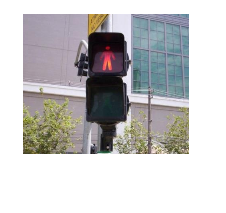
\includegraphics{figuras/semaforo_ped.PNG}}
    \caption[Semáforos]{Exemplos de sinalização semafórica.}
    \end{center}
    \label{semaforos}
\end{figure}
%http://www.cetsp.com.br/media/517462/nt252.pdf (semaforo veicular CET)(a)
%http://www.cetsp.com.br/media/478292/nt241.pdf (foco pedestres)(b)

A Figura 1.1 apresenta exemplos de sinalização semafórica, utilizados no controle de fluxos veicular (\ref{veicular}) e de pedestres (\ref{pedestre}).

Além de apresentar um sistema que realiza o controle de sinalização semafórica de maneira automatizada, também serão expostos resultados de simulações realizadas, com o intuito de demonstrar o impacto do sistema em cruzamentos de vias urbanas.

\section{Objetivo}

O objetivo desse trabalho é apresentar produtos que têm como finalidade solucionar os problemas apresentados na introdução ao assunto: gerenciamento e controle da segurança e do fluxo de veículos e pedestres nas vias urbanas. A solução apresentada é um conjunto de sistemas, com objetivos específicos cada, que, integrados, são capazes de realizar as atividades desejadas de controle de sinalização semafórica.

Além disso, serão apresentadas simulações realizadas, sob diferentes configurações do sistema, de modo a demonstrar os diferentes meios de abordagem para solucionar o problema de organização de sinalização semafórica.


\section{Estrutura do trabalho}

Esse trabalho é composto por 5 capítulos, sendo este o primeiro, e os 4 restantes são descritos, brevemente, a seguir:

\begin{itemize}
    \item Capítulo 2 - Nesse capítulo são descritas as tecnologias e fundamentações teóricas das soluções propostas
    \item Capítulo 3 - Nesse capítulo são descritos os detalhes dos sistemas implementados e como ocorre a integração entre eles
    \item Capítulo 4 - Nesse capítulo é apresentado o software utilizado para realizar as simulações e os cenários simulados
    \item Capítulo 5 - Nesse capítulo são analisados os dados obtidos das simulações
\end{itemize}
